\begin{figure}[!ht]
\centering
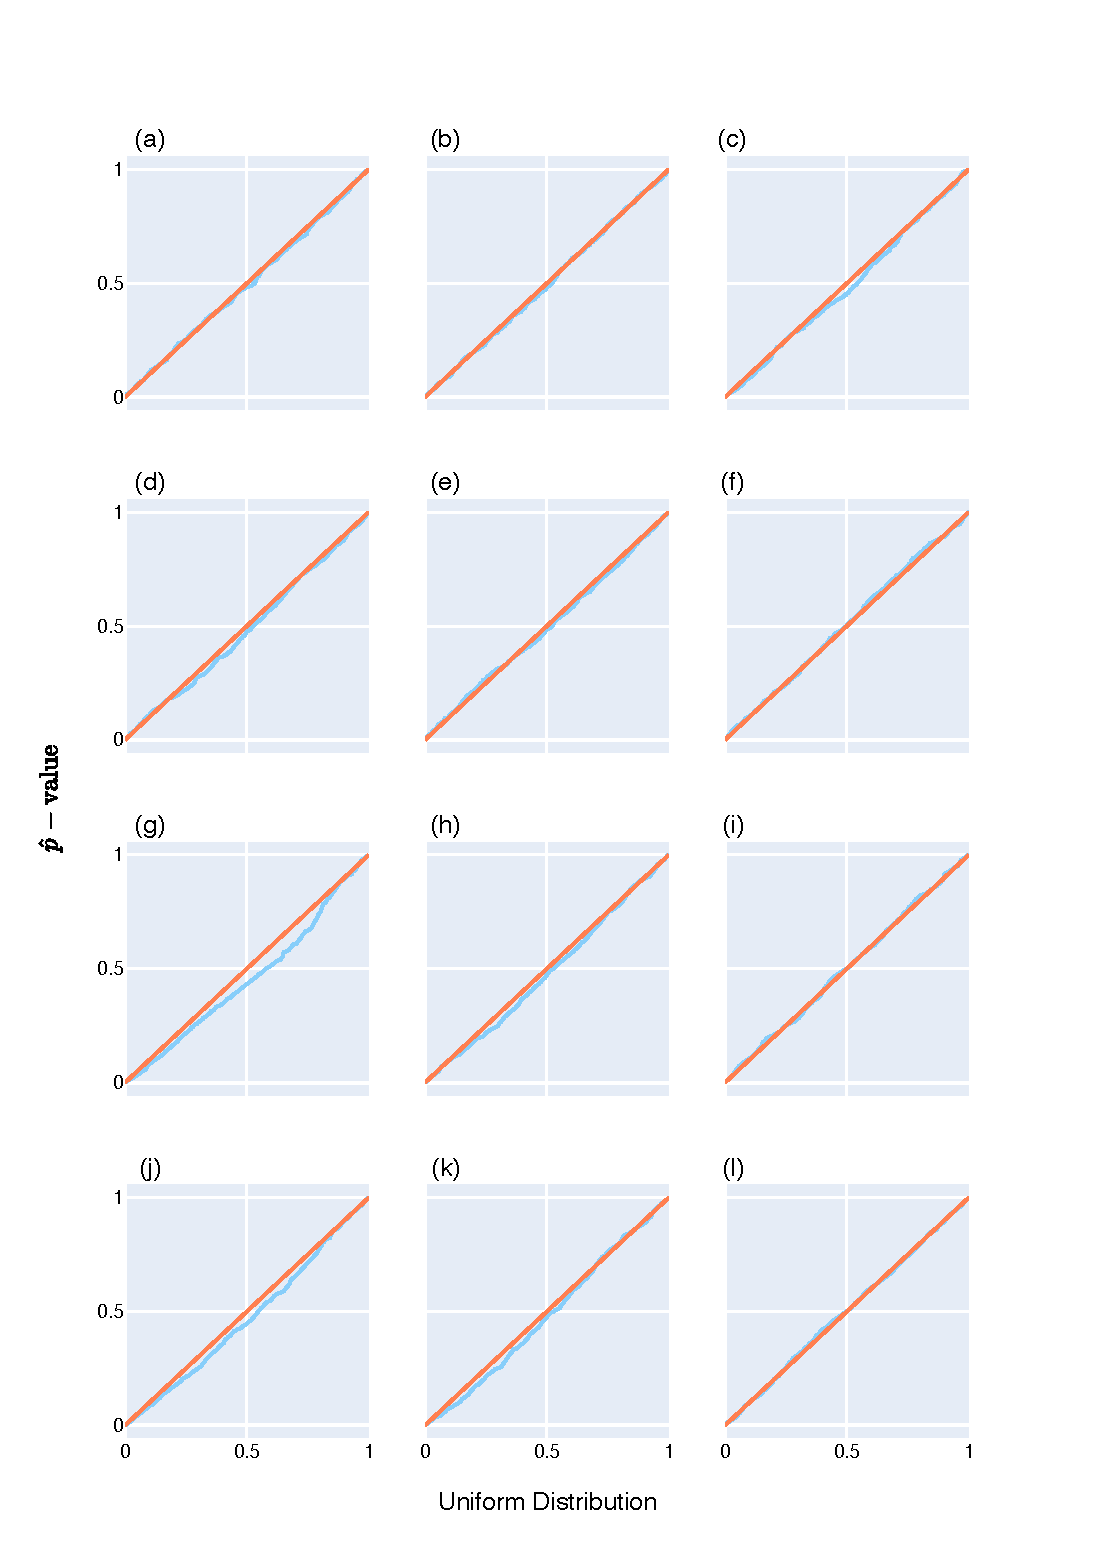
\includegraphics[width=0.8\textwidth]{figures/plots/synthetic/adj_eop/all_seeds.pdf}
\caption[The adjacent equivalence of process test is consistent with theoretical expectations for all seeds of and for alignments of all lengths]{\textbf{The adjacent equivalence of process test is consistent with theoretical expectations for all seeds of and for alignments of all lengths.} The Quantile-Quantile plots compare the distribution of $\hat p-$values to the uniform distribution. As the data points fall very close to the diagonal, this demonstrates that the distribution of $\hat p-$values is almost indistinguishable from the uniform distribution. (a), (b) and (c) show the High JSD, Low Entropy seed for alignments for length $300$, $3,000$ and $30,000$ respectively. (d), (e) and (f) show the High JSD, High Entropy seed for alignments for length $300$, $3,000$ and $30,000$ respectively. (g), (h) and (i) show the Low JSD, Low Entropy seed for alignments for length $300$, $3,000$ and $30,000$ respectively. (i), (j) and (k) shows the Low JSD, High Entropy seed for alignments for length $300$, $3,000$ and $30,000$ respectively.}
\label{fig:synthetic/adj_eop/all_seeds}
\end{figure}